% This is an ANTS2020samplepaper.tex, prepared 2020/01/20, based on 
% the Springer LNCS samplepaper.tex, a sample chapter demonstrating the
% LLNCS macro package for Springer Computer Science proceedings;
% Version 2.20 of 2017/10/04
%
\documentclass[runningheads]{llncs}
%
\usepackage{graphicx}
% Used for displaying a sample figure. If possible, figure files should
% be included in EPS format. 
% Figures should be in their original vector format (pdf, eps), if applicable. 
% Otherwise, figures provided in raster format (png, jpeg, tiff, bmp) 
% must be high-resolution (if including linework, at least 800 dpi at the
% final size, otherwise, at least 300 dpi at the final size).
%
% Although figures in the digital proceedings will be in full color, the 
% print proceedings of ANTS 2020 will be printed in grayscale. Authors should 
% therefore ensure that their figures will be appropriately legible when 
% printed in grayscale.
%
% If you use the hyperref package, please uncomment the following line
% to display URLs in blue roman font according to Springer's eBook style:
% \renewcommand\UrlFont{\color{blue}\rmfamily}

\begin{document}
	%
	% For ANTS 2020, full-length papers are strictly limited to 11 pages + references, 
	% using this template. This page limit include figures, tables, and all 
	% supplementary sections (e.g., Acknowledgements). The only exclusion from 
	% these page limits is the reference list, which should have an appropriate 
	% length with respect to the state of the art.
	%
	\title{Contribution Title}
	% Title must be capitalized according to standard “Title Case” style (i.e., all 
	% words should be capitalized, except for articles, prepositions, and conjunctions).
	%
	% Any acknowledgements should be located at the end of the paper, in a final 
	% Acknowledgements subsubsection.
	% Do not format acknowledgments as a footnote, anywhere in the paper.
	%
	\titlerunning{Abbreviated Paper Title}
	% If the paper title is too long for the running head, please set
	% an abbreviated paper title here.
	% Title must be capitalized according to standard “Title Case” style (i.e., all 
	% words should be capitalized, except for articles, prepositions, and conjunctions).
	% Do not use a \newline command with the title.
	%
	\author{First Author\inst{1}\orcidID{0000-1111-2222-3333} \and
		Second Author\inst{2,3}\orcidID{1111-2222-3333-4444} \and
		Third Author\inst{3}\orcidID{2222--3333-4444-5555}}
	% Follow the naming convention in which the surname is the last name.
	% In this field, provide the full first names (not only the initials).
	% Do not include academic titles (e.g., Prof. or Dr.).
	% Springer encourages the inclusion of author ORCIDs.
	%
	\authorrunning{F. Author et al.}
	% In this field, give the initial of the first name(s) and the full surname.
	% Give the first author's name. If there are precisely two authors, then
	% give both the first and second authors' names (sample: {F. Author and S. Author}).
	% If there are more than two authors, use ‘et al.’ after the name of the first author.
	%
	\institute{Department of Computer Science, School of Engineering and Applied Science, Princeton University, Princeton, NJ, USA \and
		Springer Heidelberg, Heidelberg, Germany
		\email{lncs@springer.com}\\ \and
		ABC Institute, Rupert-Karls-University Heidelberg, Heidelberg, Germany\\
		\email{\{abc,lncs\}@uni-heidelberg.de}}
	% Author affiliation information should include the following, using the 
	% \institute{} and \email{} fields: department, faculty, university, 
	% company (if applicable), city, country, and email address. Do not include 
	% the street address or ZIP code (ANTS 2020 does not use a postal address).
	% The email address of the corresponding author is mandatory to include in
	% the \institute{} and \email{} fields.
	%
	\index{Author, First}
	\index{Author, Second}
	\index{Author, Third}
	% After the \institute{} entries, include an \index{} entry for each author, 
	% giving the full surname, followed by the full first name(s).
	%
	\maketitle              % typeset the header of the contribution
	%
	\begin{abstract}
		The abstract should briefly summarize the contents of the paper in
		150--250 words.
		
		%ANTS 2020 does not use keywords in the proceedings.
	\end{abstract}
	%
	%
	%
	\section{First Section}
	% Section heading must be capitalized according to standard “Title Case” style 
	% (i.e., all words should be capitalized, except for articles, prepositions, 
	% and conjunctions).
	% Headings and subheadings should be aligned to the left. 
	See the LNCS Springer authors’ guidelines for details on formatting. 
	In addition, submissions must follow further requirements that are
	specific to the ANTS 2020 proceedings. These requirements are included
	in this ANTS2020samplepaper.tex template.
	
	\subsection{A Subsection Sample}
	% Subsection heading must be capitalized according to standard “Title Case” style 
	% (i.e., all words should be capitalized, except for articles, prepositions, 
	% and conjunctions).
	Please note that the first paragraph of a section or subsection is
	not indented. The first paragraph that follows a table, figure,
	equation etc. does not need an indent, either.
	
	Subsequent paragraphs, however, are indented.
	
	\subsubsection{Sample Heading (Third Level)}
	% Subsubsection heading must be capitalized according to standard “Title Case” 
	% style (i.e., all words should be capitalized, except for articles, prepositions, 
	% and conjunctions).
	Only two levels of headings should be numbered. Lower level headings 
	remain unnumbered; they are formatted as run-in headings.
	
	\paragraph{Sample Heading (Fourth Level)}
	% Paragraph heading must be capitalized according to standard “Title Case” style 
	% (i.e., all words should be capitalized, except for articles, prepositions, 
	% and conjunctions).
	The contribution should contain no more than four levels of
	headings. Table~\ref{tab1} gives a summary of all heading levels.
	
	\begin{table}[t]
		\caption{Table captions should be placed above the
			tables.}\label{tab1}
		\begin{tabular}{|l|l|l|}
			\hline
			Heading level &  Example & Font size and style\\
			\hline
			Title (centered) &  {\Large\bfseries Lecture Notes} & 14 point, bold\\
			1st-level heading &  {\large\bfseries 1 Introduction} & 12 point, bold\\
			2nd-level heading & {\bfseries 2.1 Printing Area} & 10 point, bold\\
			3rd-level heading & {\bfseries Run-in Heading in Bold.} Text follows & 10 point, bold\\
			4th-level heading & {\itshape Lowest Level Heading.} Text follows & 10 point, italic\\
			\hline
		\end{tabular}
	\end{table}
	
	For citations of references, in-text citations must use square brackets
	and consecutive numbers associated with the alphabetically ordered
	reference list at the end of the paper.
	
	When including your references using a bib file via BibTeX, please refer to
	the sample bib provided. A references list at the end of the paper will be
	automatically formatted and sorted, from the references cited with in-text 
	citations. Here is a sample of an in-text citation of a reference~\cite{sample1}, 
	and here is another~\cite{sample2}. 
	Here is a final sample~\cite{sample3,sample4,sample5}.
	% If you are not using a bib file via BibTeX, there is a sample of
	% a references list at the end of this template, with the mandatory
	% formatting. For this sample reference list,
	% the following bibliography provides
	% a sample reference list with entries for journal
	% articles~\cite{ref_article1}, an LNCS chapter~\cite{ref_lncs1}, a
	% book~\cite{ref_book1}, proceedings without editors~\cite{ref_proc1},
	% and a homepage~\cite{ref_url1}. Multiple citations are grouped
	% \cite{ref_article1,ref_lncs1,ref_book1},
	% \cite{ref_article1,ref_book1,ref_proc1,ref_url1}.
	
	\noindent Displayed equations are centered and set on a separate
	line.
	\begin{equation}
	x + y = z
	\end{equation}
	Please try to avoid rasterized images for line-art diagrams and
	schemas. Whenever possible, use vector graphics instead (see
	Fig.~\ref{fig1}).
	
	\begin{figure}[h]
		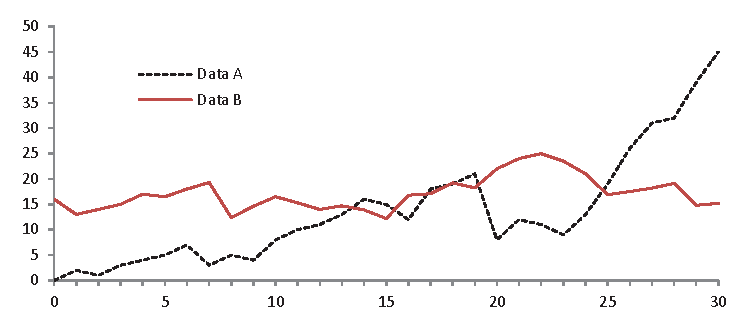
\includegraphics[width=\textwidth]{fig1.eps}
		\caption{A figure caption is always placed below the illustration.
			Please note that short captions are centered, while long ones are
			justified by the macro package automatically.} \label{fig1}
	\end{figure}
	
	\begin{theorem}
		This is a sample theorem. The run-in heading is set in bold, while
		the following text appears in italics. Definitions, lemmas,
		propositions, and corollaries are styled the same way.
	\end{theorem}
	%
	% the environments 'definition', 'lemma', 'proposition', 'corollary',
	% 'remark', and 'example' are defined in the LLNCS documentclass as well.
	%
	\begin{proof}
		Proofs, examples, and remarks have the initial word in italics,
		while the following text appears in normal font.
	\end{proof}
	
	\subsubsection*{Acknowledgements}
	Acknowledgements, if applicable, should be given here as the last 
	subsubsection of the paper, just before the list of references.
	% Do not format acknowledgments as a footnote, anywhere in the paper.
	%
	% ---- Bibliography ----
	%
	% When using BibTeX, use bibliography style 'splncs04'.
	% References will then be sorted and formatted in the correct style.
	%
	\bibliographystyle{splncs04}
	\bibliography{mybibliography}
	%
	% Below is a bibliogrpahy sample using the mandatory style, if not you 
	% choose to not use a bib file via BibTeX.
	% 
	% \begin{thebibliography}{8}
	% \bibitem{ref_article1}
	% Author, F.: Article title. Journal \textbf{2}(5), 99--110 (2016)
	
	% \bibitem{ref_lncs1}
	% Author, F., Author, S.: Title of a proceedings paper. In: Editor,
	% F., Editor, S. (eds.) CONFERENCE 2016, LNCS, vol. 9999, pp. 1--13.
	% Springer, Heidelberg (2016). \doi{10.10007/1234567890}
	
	% \bibitem{ref_book1}
	% Author, F., Author, S., Author, T.: Book title. 2nd edn. Publisher,
	% Location (1999)
	
	% \bibitem{ref_proc1}
	% Author, A.-B.: Contribution title. In: 9th International Proceedings
	% on Proceedings, pp. 1--2. Publisher, Location (2010)
	
	% \bibitem{ref_url1}
	% LNCS Homepage, \url{http://www.springer.com/lncs}. Last accessed 4
	% Oct 2017
	% \end{thebibliography}
	%
\end{document}